\documentclass[Bachelorarbeit.tex]{subfiles}
\begin{document}

\newpage
\section{Results}
\label{Results}
In the following section, results of testing are presented. First, an evaluation of each step, the comparison of parameters for each key point detection algorithm, Lucas-Kanade optical flow and preprocessing is analyzed, with a main focus on the low level measures average lifespan and number of tracked points. A threshold for the latter is set at 500 points over 10.000 frames and the parameter-settings with the highest average lifespan over this threshold are chosen for further testing. Initially, an educated guess for parameters of Lucas-Kanade and preprocessing were chosen. 

Thereafter, having compared each setting on these simple measures, insight is given for more sophisticated measures explained in \autoref{setup}.

\subsection{Comparison by Average Lifespan and Quantity}

\subsubsection{Key Point Detection Algorithms}

\begin{center}
	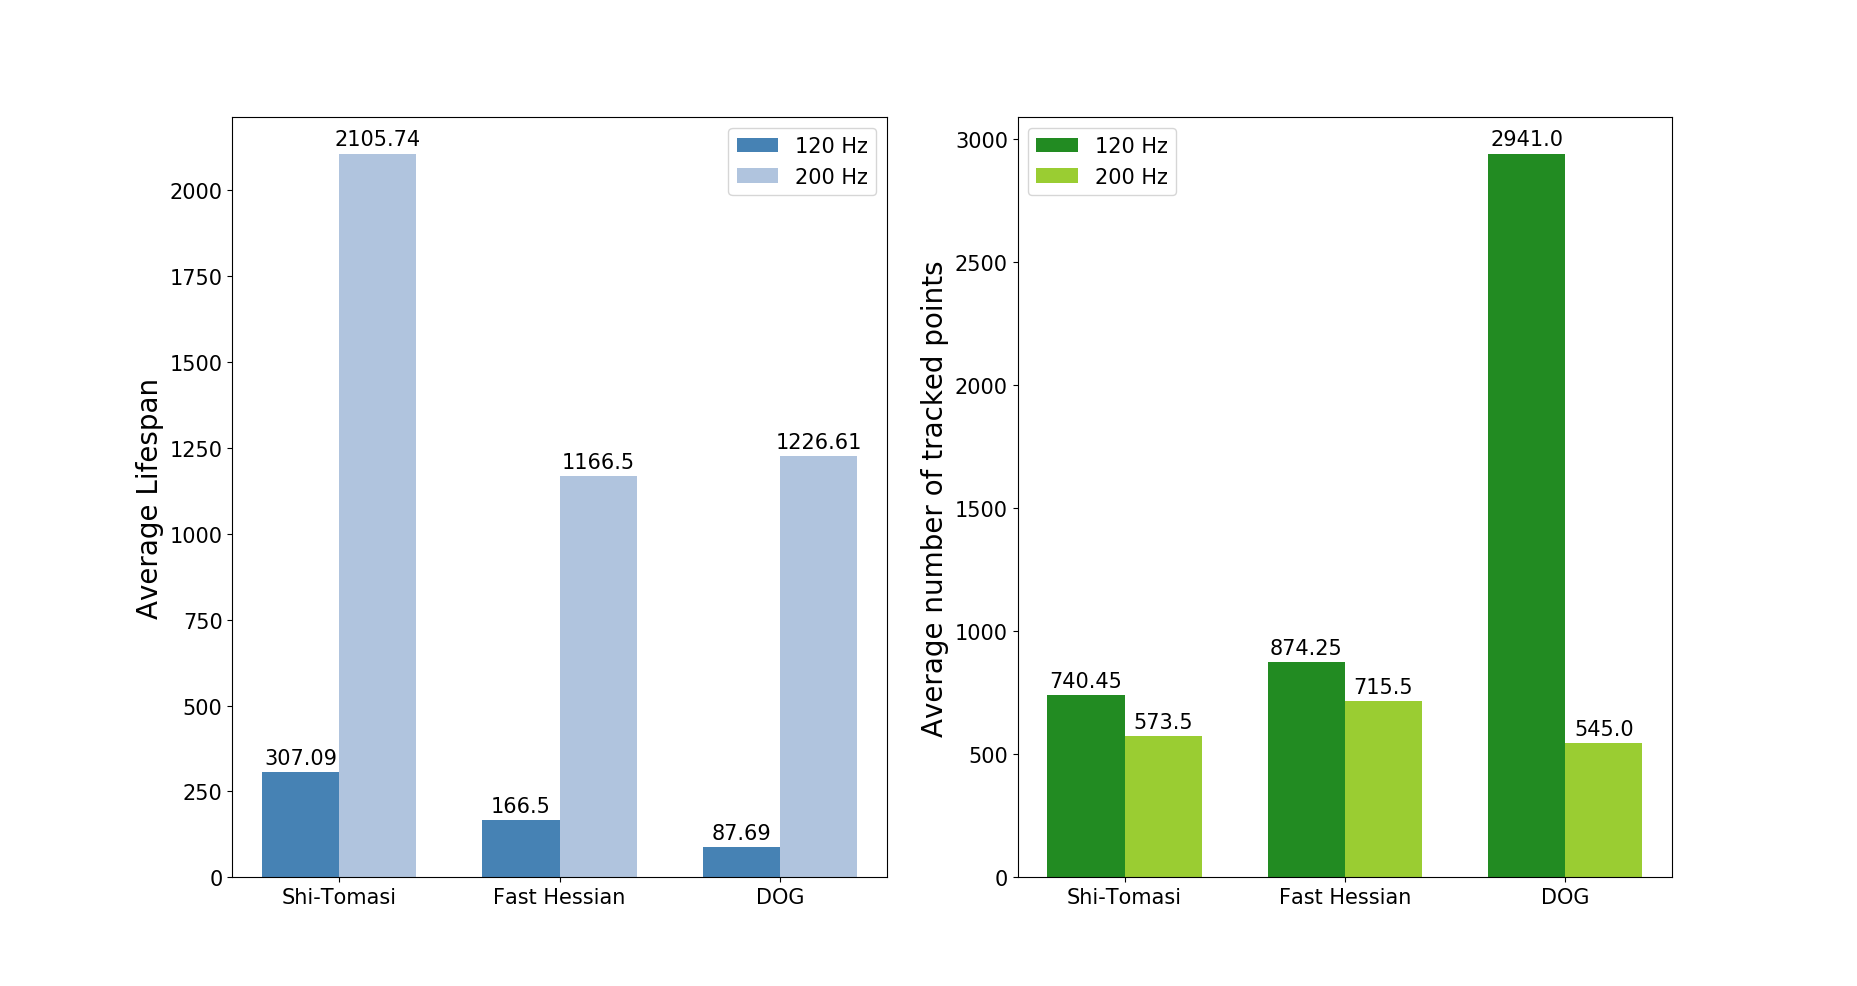
\includegraphics[width=1.1\linewidth]{Images/values_keypointdetectors}
	\captionof{figure}{Values of best settings for each key point detector, averaged over all videos in the respective framerate} 
	\label{detectors_120_200}
\end{center}

When comparing the average lifespan of various settings, the most remarkable result is the difference between the videos taken by cameras with a frame-rate of 120 Hz and those with 200 Hz. All key point detectors show a notable higher lifespan and a lower number of tracked points for this increase in frame rate and lower resolution, as can be seen in \autoref{detectors_120_200}. This becomes particularly apparent by comparing the key point parameter settings with the highest average lifespan. The Shi-Tomasi detector shows an average lifespan of 307.09 for its 740.45 tracked points in videos with 120 fps, while the 573.50 tracked points in videos with 200 fps yield an average lifespan of 2105.74. Similarly are the results of the fast Hessian detector: 874.25 points tracked with and average lifespan of 166.50 for 120 Hz videos, and 1166.50 for 715.50 tracked points in videos with 200 fps. Comparatively, if somewhat more extreme, are the values found for the DoG detector: 2941 tracked points with an average lifespan of 87.69 frames were the results of the tests with 120 fps, while it shows 545 tracked points with an average lifespan of 1226.61 for videos with 200 Hz.\\
Furthermore it is visible that the Shi-Tomasi corner detector shows the highest average lifespan of the three detectors, for both classes of videos. The second highest yields the fast Hessian detector and the DoG method comes third. The average number of tracked points, on the other hand, shows as vast maximum of tracked points for the DoG method in videos with 120 fps, it is more than doubling the amounts of the Shi-Tomasi and fast Hessian detectors. The latter had the most tracked points on average for the 200 Hz videos, while 
Shi-Tomasi is in the middle, with DoG being the lowest in this measure.

%The Shi-Tomasi detector shows the best performance in these measures especially concerning the videos with 120 fps. Its best parameter setting has an average lifespan over all videos of 307.09 frames with 740.45 points being tracked on average. Its best setting has the second longest average lifespan (2717.08) in videos with 200 fps after the difference of Gaussian detector (4351.5), with the fast Hessian detector (2114.89) in third place. This is not considering the number of tracked points, in which one can see a drawback of the high lifespan of the DoG detector. There is only one tracked key point for the videos with 200 Hz for the best setting, while fast Hessian comes to 9 on and the Shi-Tomasi detector to 152.5 frames on average, per video. This relation of tracked points is also illustrated in videos with 120 fps, but not to such an extend. Also here comparison is made for the settings with the highest average lifespans: The Shi-Tomasi detector has the most number of tracked points, with an average of 740.45 per video. Relative to it, the fast Hessian and DoG detectors have a low number of 233.4 and 240.15, respectively. 

%The Fast Hessian key point detector performs worst in the videos with 200 fps, but is in second place for videos with the lower frame-rate. Interestingly, the difference of Gaussian approach shows the worst performance concerning average lifespan in 120 fps videos, but the best in 200 fps videos. The runtime is much lower in both classes of videos for the Shi-Tomasi detector than the other two, which show no significant difference in the one with lower frame-rate. The difference of Gaussian detector is also a bit faster in detection in videos with 200 fps compared to the fast Hessian approach.\\

%When looking at the average number of tracked key points over all videos, the differences are even greater. 
When viewing parameter-settings of the three algorithms, the difference between videos with 120 and 200 fps persist. On this account, analysis of the results is 

When looking at different values for parameter-settings of each algorithm, beginning with the Shi-Tomasi corner detector, differences between videos with 120 and 200 fps persist. A medium quality level yields high values for average lifespan as does a large distance between corner points for those recorded with 120 Hz. Also, large neighborhoods to calculate the covariation matrix proves to be more successful than smaller ones. 
For videos recorded at 200 Hz, a high quality level, medium to large minimal distance between key points and a small size for the covariation matrix prove to be more successful. Furthermore, the restriction by a maximum of detected corners does not seem to change a lot in average lifespan in both classes of videos, but does so in the number of tracked points. Also the quality level is of importance here - the setting with the lowest tested quality level and the highest tested maximum of returned corners yields an average of 168206.45 and 15893 key points per video, accompanied with the lowest average lifespan of this test, 65.02 and 408.14 for videos with 120 fps and 200 fps, respectively.\\

For the fast Hessian detector, low numbers for octaves, octave-layers and the Hessian threshold yield a high lifespan for videos with 120 fps. Quite the opposite is the case for video with a higher frame-rate: high numbers of octave layers and a medium threshold proves to be superior. For settings with various number of octaves, the same results concerning average lifespan and number of tracked points is visible, as is the case for higher numbers of octaves in videos with 120 fps. The highest key points tracked is with a setting of highest number of octaves and octave layers and the lowest number for the Hessian threshold.

The DoG detector shows the best average lifespan in 120 Hz videos with a setting of a high value for sigma and low values for number of features, octave layers and both thresholds. What is visible overall for this class of videos, is that low thresholds for contrast and edges perform best, while these settings of the latter did not prevail the thresholding of average number of tracked points in videos with 200 fps. In these, a low value for sigma is superior. A low number of features improve the average lifespan, but lessen the number of key points, which is showing in both classes of videos. Furthermore yields a setting with many octave layers better results in both measures, average lifespan and number of tracked points, over both classes of videos. The highest number of tracked points is returned, when setting sigma and contrast threshold to low values, with high values for the returned number of features and edge threshold. The settings for the two classes of videos differ only in the setting for the number of octave layers, which is the lowest for 200 fps videos and highest for those with 120 fps.
%For the fast Hessian detector, the longest average lifespan of 211.21 per video yields a combination of parameters with just one octave and only one octave layer and a moderately small Hessian threshold of 100. The number of tracked key points, on the other hand, is very low for this setting, with only a value of 233.4. In general, combinations with a low number of octaves and octave layers seem to offer a high average lifespan.  Opposed to this, the number of tracked points is large for a low Hessian threshold, many octaves and octave-layers. The maximum is 88509.65 on average per video (120 fps), this setting is accompanied by a low average lifespan of 43.32.\\ 


%For the difference of Gaussian approach, the highest average lifespan (114.43) is reached by high values for contrast threshold and sigma, a moderate amount of octave layers and a low value for edge threshold and number of features. This parameter setting is accompanied by a very low value for number of tracked points, 240.15 on average per video with 120 fps. The maximum of tracked points on average (24081.25 for 120 fps) is reached, by setting the contrast threshold and sigma very low, additional to a high edge threshold, number of octave layers and features. This setting reaches a moderate value for average lifespan, 54.83 for the videos with 120 fps, compared to the other parameter settings of DoG.


\subsubsection{Parameters for the Lucas-Kanade Algorithm}
For the evaluation of parameters for the Lucas-Kanade optical flow algorithm, the parameter-settings for each key point detector with the highest average lifespan over the threshold of 500 tracked points on average per video were chosen in respect to the class of videos, coming to a total of 6 settings. 

\begin{center}
	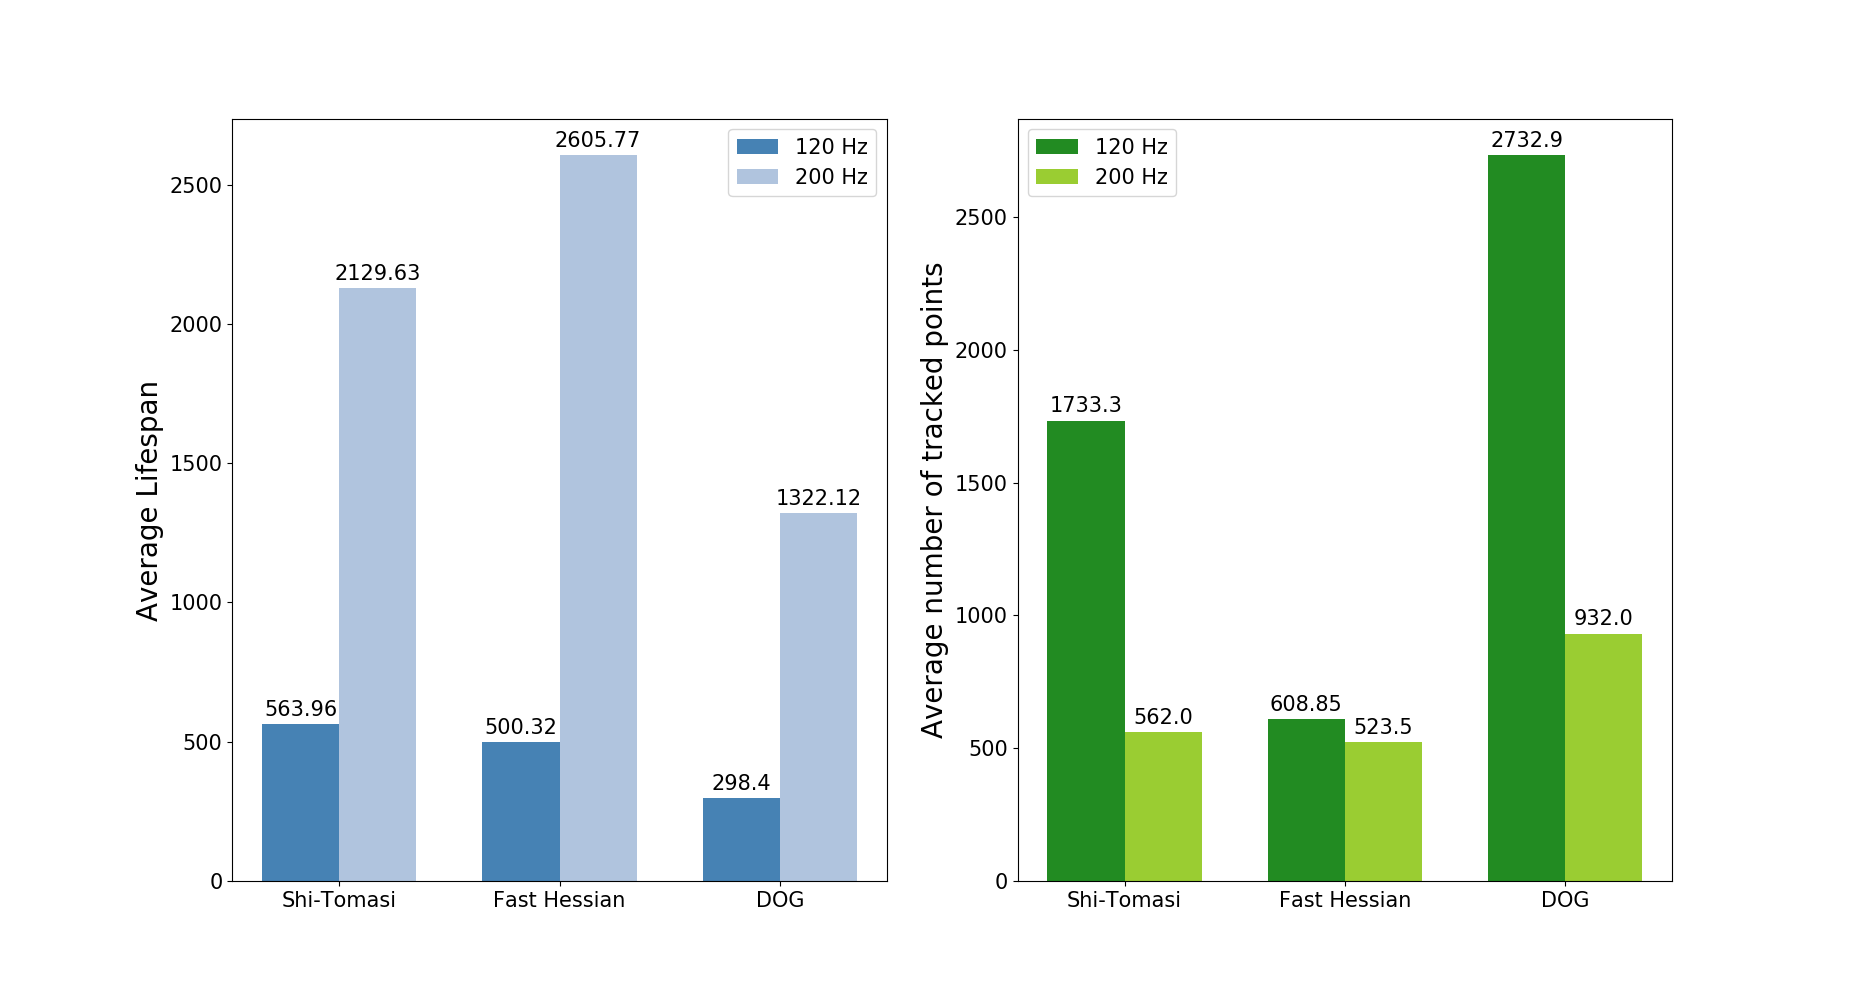
\includegraphics[width=1.1\linewidth]{Images/values_lk}
	\captionof{figure}{Values of best settings for each key point detector and the Lucas-Kanade algorithm, averaged over all videos in the respective framerate} 
	\label{lk_120_200}
\end{center}

As is visible in \autoref{lk_120_200}, the differences for the two classes of videos persist. For those with a frame-rate of 120 Hz, the best setting of parameters for Lucas-Kanade optical flow and the Shi-Tomasi detector yield an average lifespan of 563.96, while the result for 200 Hz videos is nearly four times as much, 2129.63. The number of tracked points, on the other hand, is much lower for videos with the higher frame-rate, than for the lower one, 562 and 1733.3, respectively. The behavior for the best setting of Lucas-Kanade parameters in respect to the best settings for the DoG method is similar. For 120 fps videos, the resulting values of average lifespan are 298.4 and 1322.12 for those taken with 200 Hz. Also the number of tracked points are on average per video 2732.9 and 932.0 for lower and higher frame-rate, respectively. While the fast Hessian detector shows similar results for the average lifespan as the other two detectors, 500.32 (120 Hz) and 2605.77 (200 Hz), the number of tracked points shows a difference: It returns only 608.85 on average for videos with 120 fps, which is only less than 20 percent more, than for videos with a higher frame-rate. Both of these yield the lowest result in comparison to the other two detectors.\\

The best parameter settings for Lucas-Kanade optical flow are equal in all key points detectors for videos with a frame-rate of 120. A large window size, a high value for the epsilon\todo{was is das genau?} and a low one for the maximal number of iterations proves to be the best setting of Lucas-Kanade concerning average lifespans over all 120 fps videos. The setting of differing values for the maximum number of levels of reduction yields only a difference between low and medium/high numbers. The outcome is the same for a setting of 3 and 10 for this value, which also holds true concerning the videos with a higher frame-rate. The parameter-settings for the Lucas-Kanade algorithm differ more for the highest outcome of average lifespan per detector over the videos with that frame-rate. The value is highest for the fast Hessian detector, with a medium window size, a medium/high number of maximum level of reduction and a low value for epsilon. The only difference in the setting for the Shi-Tomasi detector is the window size, which is better with a medium value. The same value proves to be superior for the DoG method for key point detection, in addition to a high value for epsilon and the lowest setting for the number of iterations and maximum level of reduction.\\
In general, it can be said that a large window size yields higher average lifespans, as does more than one level of reduction, excluding the results of the DoG method for 200 Hz videos. The termination criteria show a lower value of average lifespan for a high number of maximum iteration and a low value for epsilon and high one for vice versa. A medium average lifespan is accounted for medium numbers of termination criteria. \todo{vlt nochmal genauer anschauen}\\
The number of tracked points is highest for the DoG detector and a small window size, a large level of reduction and medium value for the termination criteria of iteration and a low one for epsilon. It is accompanied by the lowest average lifespan, 20.95 for 120 hz videos and 153.09 for 200 Hz videos. It declines for a larger window size and higher values for both termination criteria. This holds true for both classes of videos and all detectors.

\subsubsection{Parameters for Preprocessing}

\begin{center}
	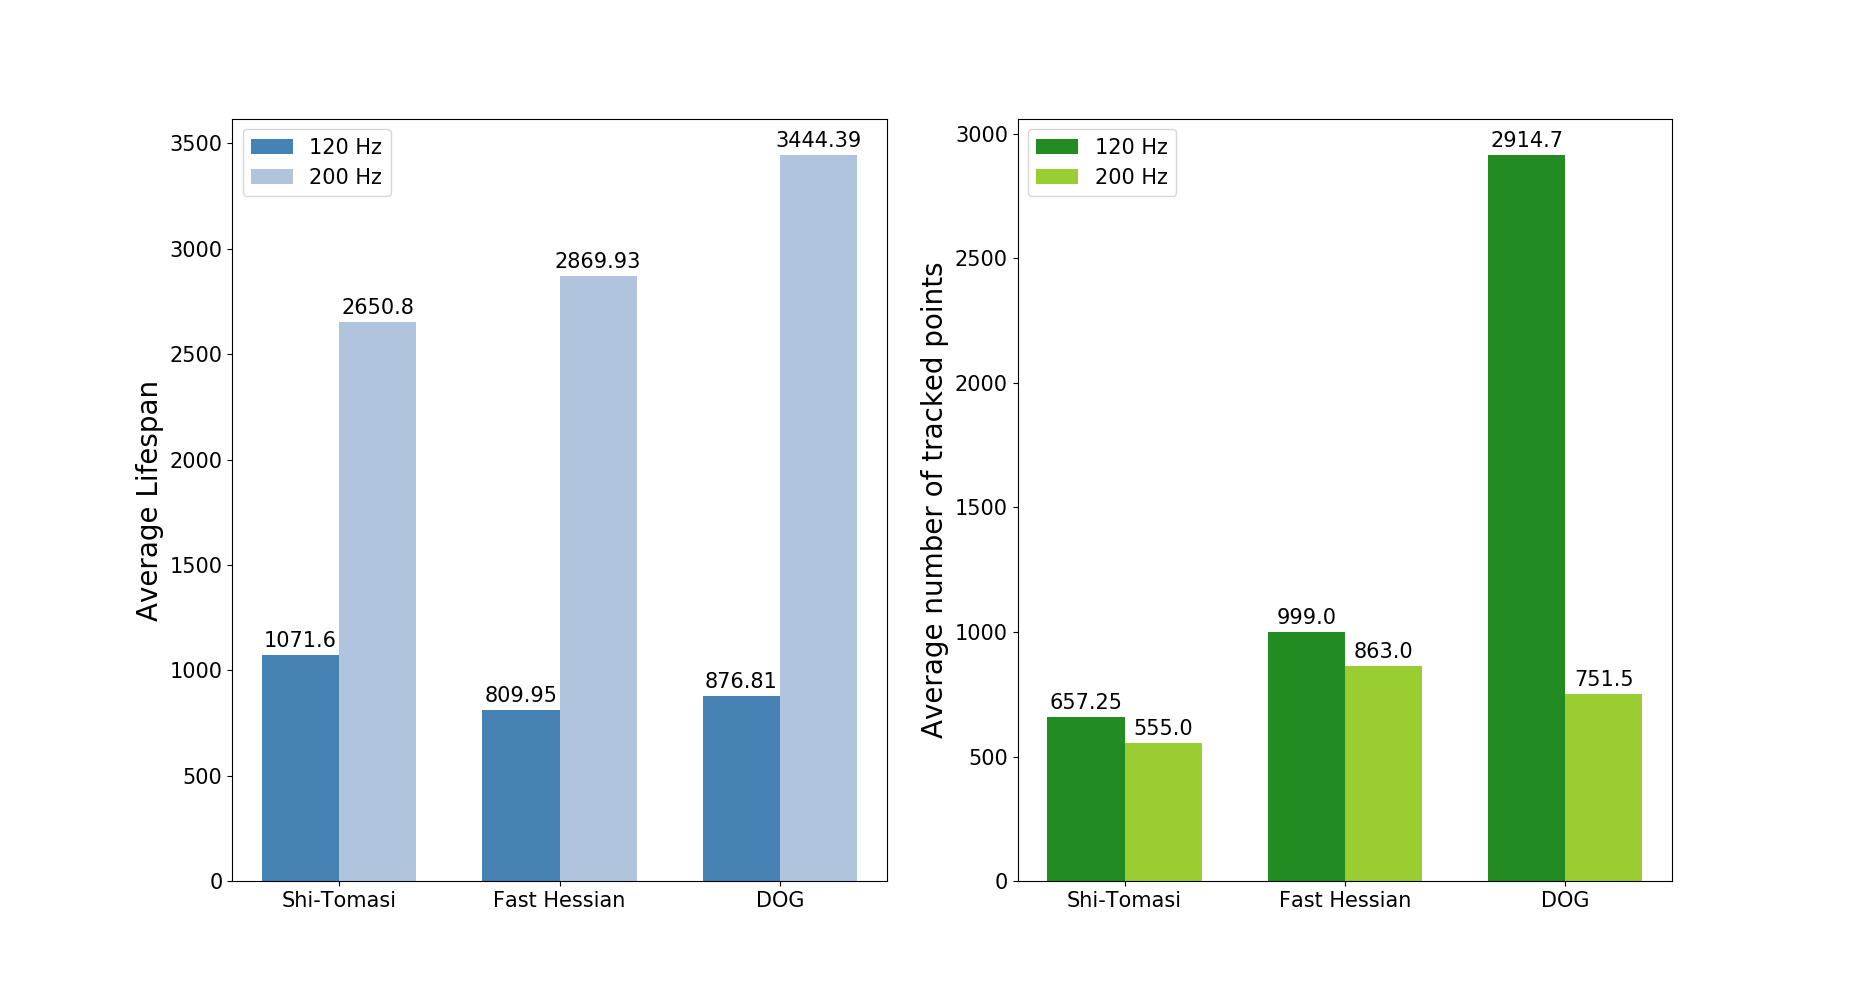
\includegraphics[width=1.1\linewidth]{Images/values_prep}
	\captionof{figure}{Values of best settings for each key point detector and the Lucas-Kanade algorithm, averaged over all videos in the respective framerate} 
	\label{prep_120_200}
\end{center}





\FloatBarrier
\end{document}